\documentclass{article}

\usepackage{graphicx}
\usepackage{tikz}
\usepackage{tikzsymbols}
\usetikzlibrary{calc,patterns,shapes.geometric}
\pagestyle{empty}
\usepackage[margin=0pt]{geometry}
\geometry{papersize={14in,12in}}

\def\centerarc[#1](#2)(#3:#4:#5){\draw[#1] ($(#2)+({#5*cos(#3)},{#5*sin(#3)})$) arc (#3:#4:#5);}

\begin{document}
	\begin{figure}
		\centering
		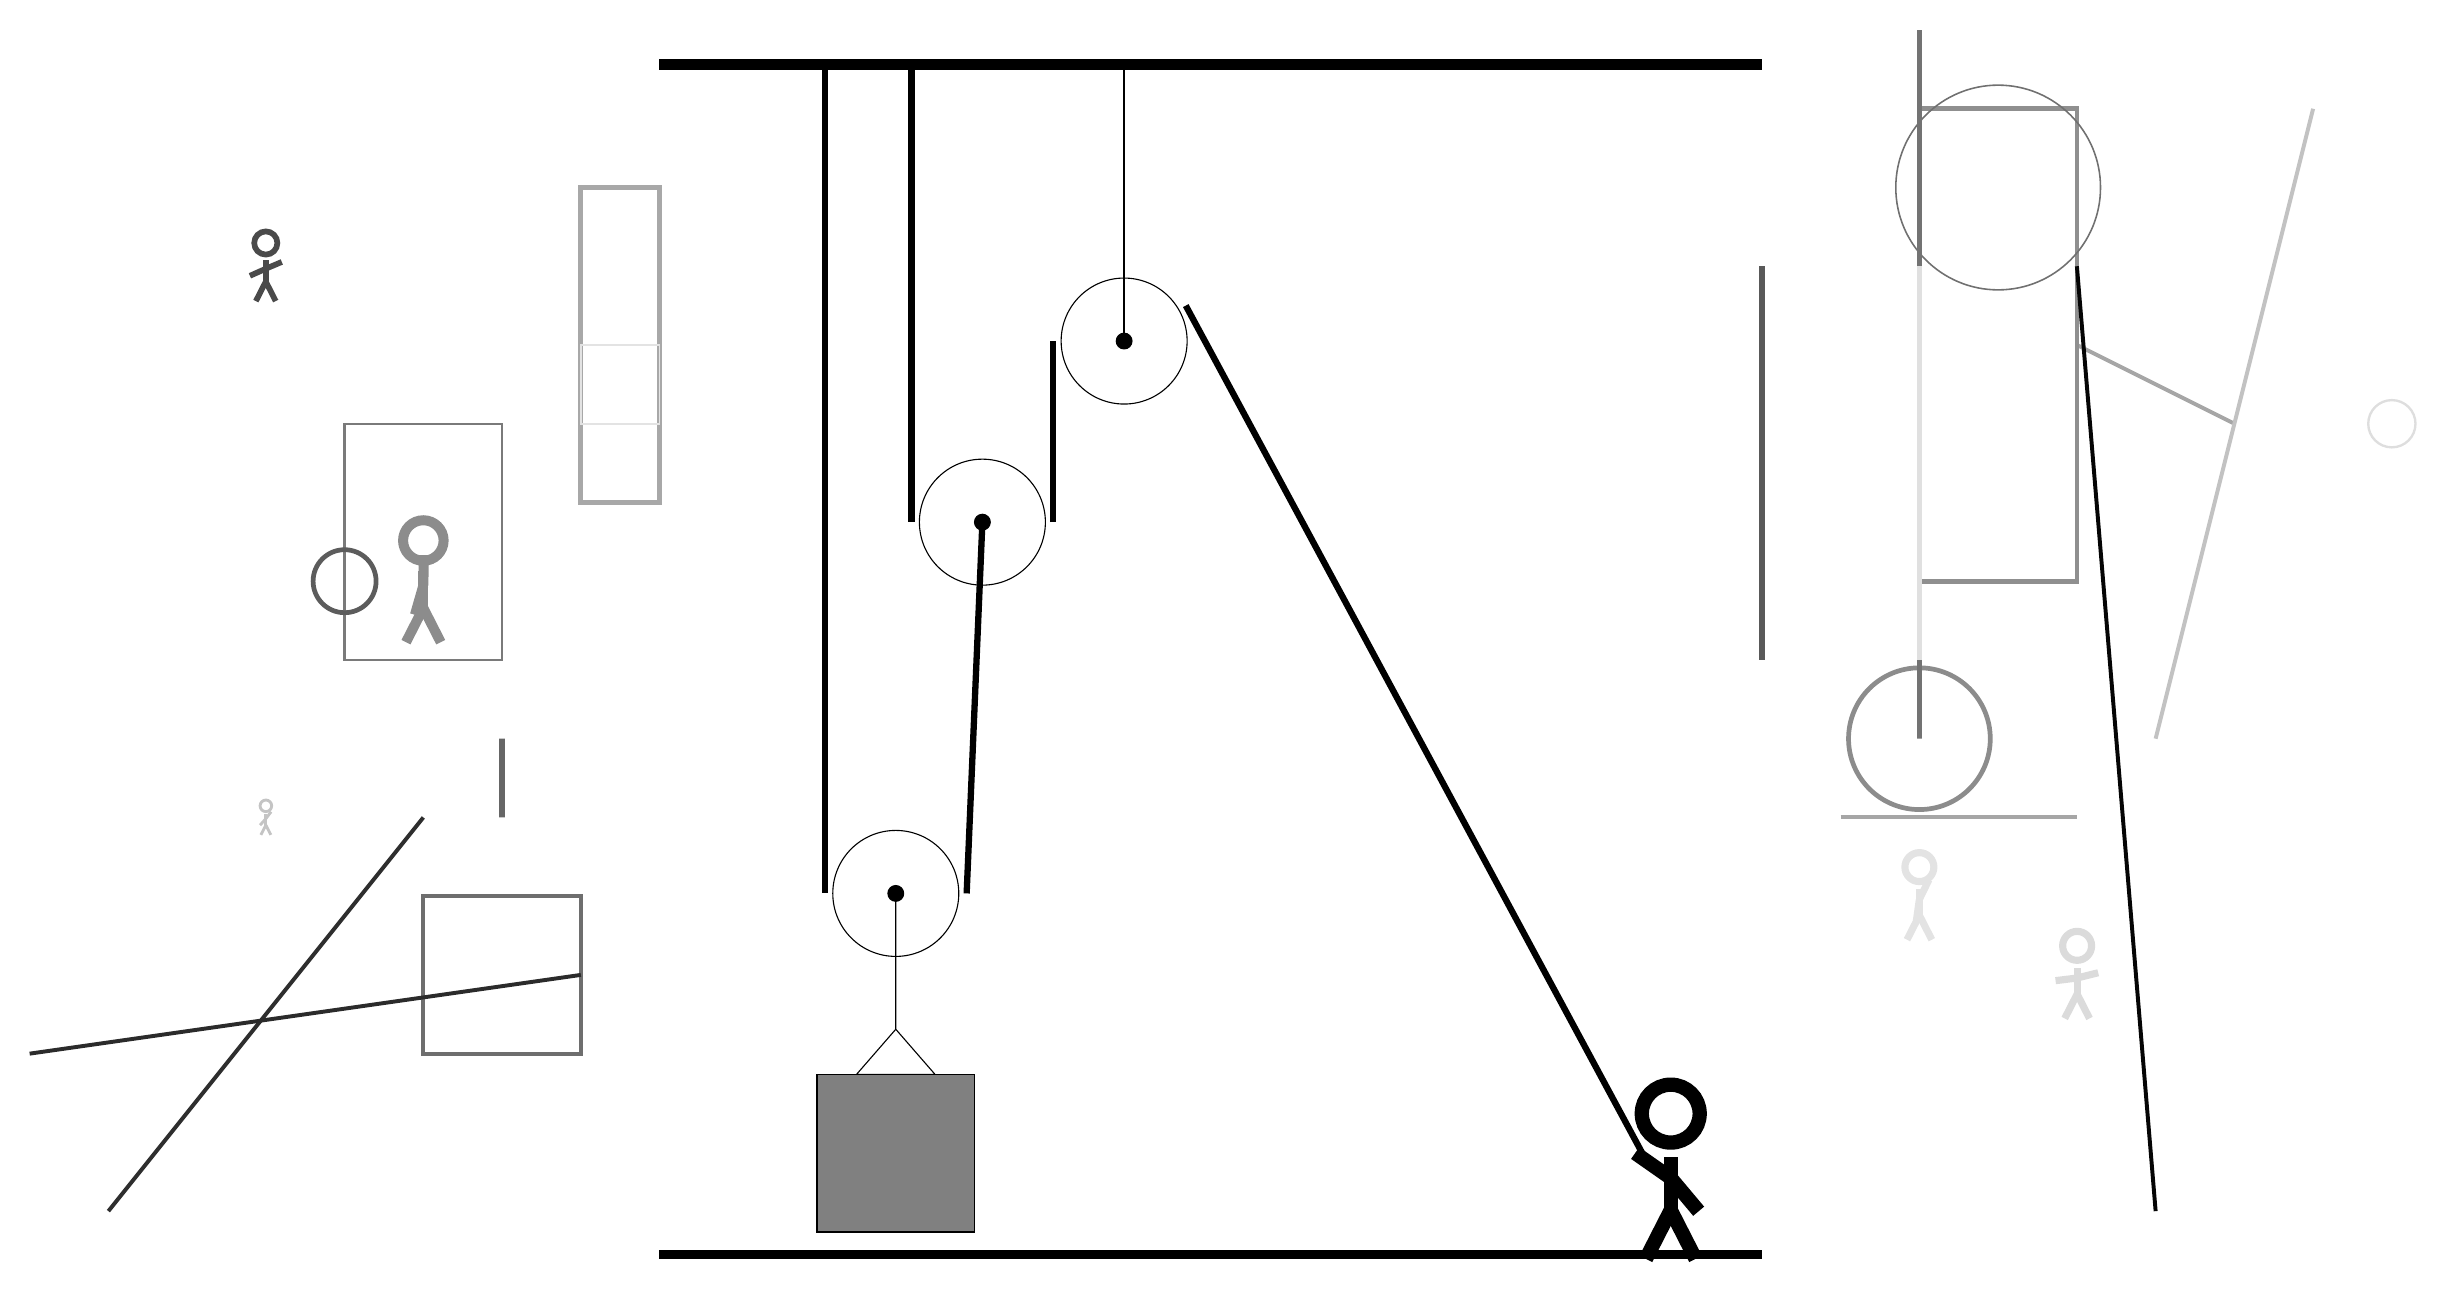
\begin{tikzpicture}
			%%%%% START %%%%%
			
			\draw[fill=black] (-2, 11.5) rectangle (12, 11.625);
			
			\draw[line width=0.6mm, color=black!34] (-2, 10) rectangle (-3, 6);
			
			\draw[line width=0.7mm, color=black!60] (-4, 3) rectangle (-4, 2);
			\node[line width=0.4mm, color=black!11] at (14, 1) {\Strichmaxerl[5][82][64]};
			\draw[line width=0.5mm, color=black!35](16, 8) -- (18, 7);
			\node[line width=0.6mm, color=black!14] at (16, 0) {\Strichmaxerl[5][7][14]};
			\draw[line width=0.5mm, color=black!57] (-3, 1) rectangle (-5, -1);
			
			\draw[line width=0.6mm, color=black!44] (14, 5) rectangle (16, 11);
			\draw[line width=0.3mm, color=black!52] (-4, 4) rectangle (-6, 7);
			\draw[line width=0.5mm, color=black!82](-5, 2) -- (-9, -3);
			\draw[line width=0.5mm, color=black!83](-3, 0) -- (-10, -1);
			
			\draw[line width=0.2mm, color=black!11] (-3, 8) rectangle (-2, 7);
			
			\draw[line width=0.5mm, color=black!35](13, 2) -- (16, 2);
			\draw [line width=0.2mm, color=black!56](15, 10) circle (1.3);
			\draw[line width=0.5mm, color=black!98](17, -3) -- (16, 9);
			\draw [line width=0.6mm, color=black!64](-6, 5) circle (0.4);
			\draw [line width=0.3mm, color=black!13](20, 7) circle (0.3);
			
			\draw [line width=0.6mm, color=black!45](14, 3) circle (0.9);
			
			\draw[line width=0.7mm, color=black!65] (12, 9) rectangle (12, 4);
			\draw[line width=0.6mm, color=black!55] (14, 3) rectangle (14, 12);
			\node[line width=0.3mm, color=black!45] at (-5, 5) {\Strichmaxerl[7][74][89]};
			\node[line width=0.3mm, color=black!23] at (-7, 2) {\Strichmaxerl[2][48][53]};
			\draw[line width=0.5mm, color=black!24](17, 3) -- (19, 11);
			\node[line width=0.7mm, color=black!71] at (-7, 9) {\Strichmaxerl[4][24][23]};
			\draw[line width=0.6mm, color=black!12] (14, 4) rectangle (14, 9);
			
			\draw (1, 1.035) circle (0.8);
			\draw[fill=black] (1, 1.035) circle (0.1);
			
			\draw (2.1, 5.75) circle (0.8);
			\draw[fill=black] (2.1, 5.75) circle (0.1);
			
			\draw (3.9, 8.05) circle (0.8);
			\draw[fill=black] (3.9, 8.05) circle (0.1);
			\draw[thick] (3.9, 8.05) -- (3.9, 11.5);
			
			\draw (1, 1.035) -- (1, -0.69) -- (0.5, -1.265) -- (1.5, -1.265) -- (1, -0.69);
			\draw[fill=black!50] (0, -1.265) rectangle (2, -3.265);
			
			\draw[line width=0.8mm] (0.1, 11.5) -- (0.1, 1.035);
			\centerarc[line width=0.8mm](1, 1.035)(180:360:0.9);
			\draw[line width=0.8mm](1.9, 1.035) -- (2.1, 5.75);
			\draw[line width=0.8mm] (1.2, 11.5) -- (1.2, 5.75);
			\centerarc[line width=0.8mm](2.1, 5.75)(180:360:0.9);
			\draw[line width=0.8mm](3.0, 5.75) -- (3.0, 8.05);
			\centerarc[line width=0.8mm](3.9, 8.05)(30:180:0.9);
			\draw[line width=0.8mm] (4.683, 8.5) -- (10.5, -2.3);
			
			\node at (10.8, -2.5) {\Strichmaxerl[10][-35][-50]};
			
			\draw[fill=black] (-2, -3.5) rectangle (12, -3.6);
			
			%%%%% END %%%%%
		\end{tikzpicture}
	\end{figure}	
\end{document}